%%%%%%%%%%%%%%%%%%%%%%%%%%%%%%%%%%%%%%%%%%%%%%%%%%%%%%
\begin{frame}[c]{ }
	\frametitle{Map Reduce Components }
	
	The Map-Reduce consists of three "main" parts
	
	\begin{itemize}  [<+->]
		\item [--] The Driver.
		\item [--] The Mapper.
		\item [--] The Reducer.
		
	\end{itemize}
\end{frame}

%%%%%%%%%%%%%%%%%%%%%%%%%%%%%%%%%%%%%%%%%%%%%%%%%%%%%%
\begin{frame}
	
	\begin{figure}
		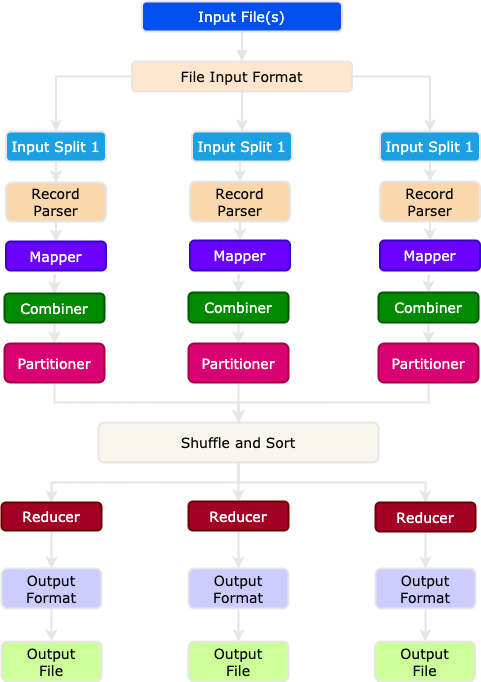
\includegraphics[height=.925\textheight]{./Figures/chapter-02/Map-Reduce.png}
		\caption{Map Reduce Stages } \label{fig:MRSteps}
	\end{figure}			
\end{frame}
%%%%%%%%%%%%%%%%%%%%%%%%%%%%%%%%%%%%%%%%%%%%%%%%%%%%%%
\begin{frame}
	
	\begin{figure}
		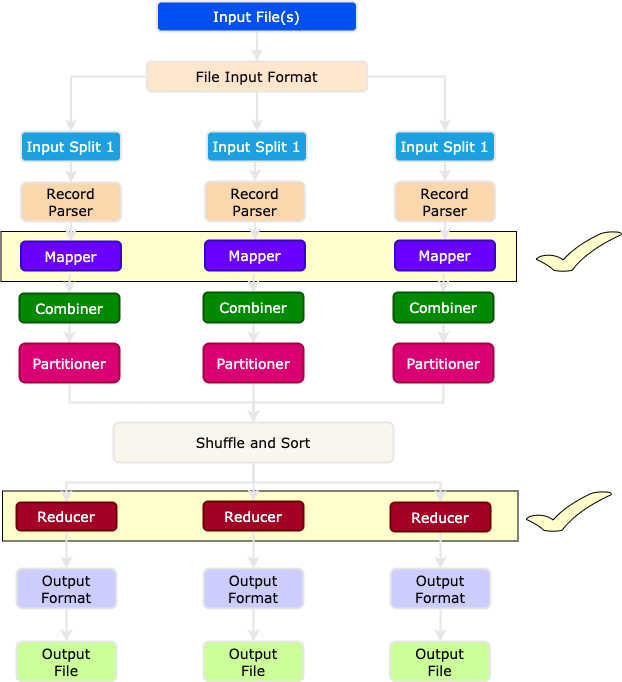
\includegraphics[height=.925\textheight]{./Figures/chapter-02/Map-Reduce_2.png}
		\caption{Map Reduce Stages } \label{fig:MRSteps2}
	\end{figure}			
\end{frame}
%%%%%%%%%%%%%%%%%%%%%%%%%%%%%%%%%%%%%%%%%%%%%%%%%%%%%%
\begin{frame}
	
	\begin{figure}
		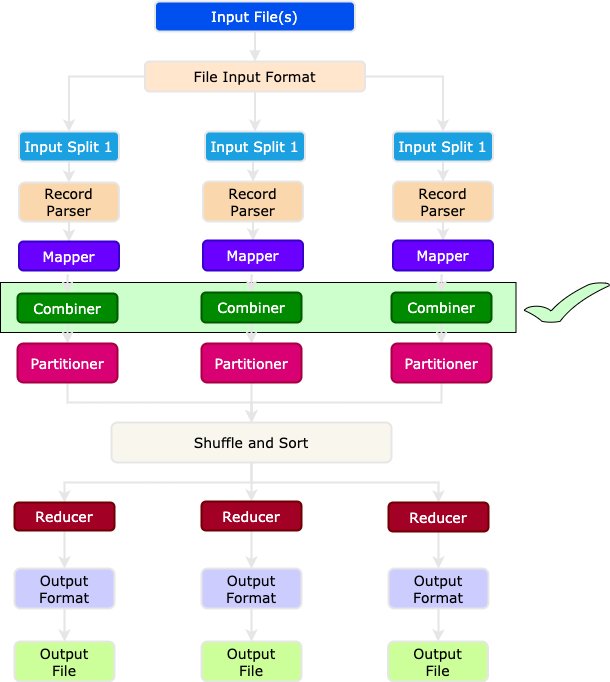
\includegraphics[height=.925\textheight]{./Figures/chapter-02/Map-Reduce-components-combiner.png}
		\caption{Map Reduce Stages } \label{fig:MRSteps2}
	\end{figure}			
\end{frame}

%%%%%%%%%%%%%%%%%%%%%%%%%%%%%%%%%%%%%%%%%%%%%%%%%%%%%%
\begin{frame}[c]{ }
	\frametitle{ The Combiners}
	\centering     
	
	\textcolor{offgreen}{ \large Increase The Map-Reduce Processing Using The Combiners}
\end{frame}
%%%%%%%%%%%%%%%%%%%%%%%%%%%%%%%%%%%%%%%%%%%%%%%%%%%%%%
\begin{frame}
	
	\begin{figure}
		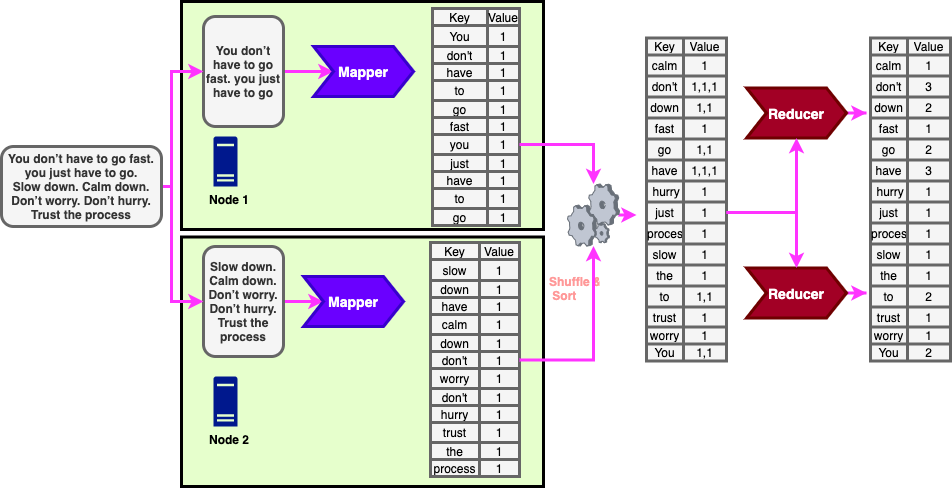
\includegraphics[height=.85\textheight]{./Figures/chapter-02/map-reduce-combiner-ex-1.png}
		\caption{Map Reduce Without Combiner } \label{fig:MRCombiner1}
	\end{figure}			
\end{frame}
%%%%%%%%%%%%%%%%%%%%%%%%%%%%%%%%%%%%%%%%%%%%%%%%%%%%%%
\begin{frame}
	
	\begin{figure}
		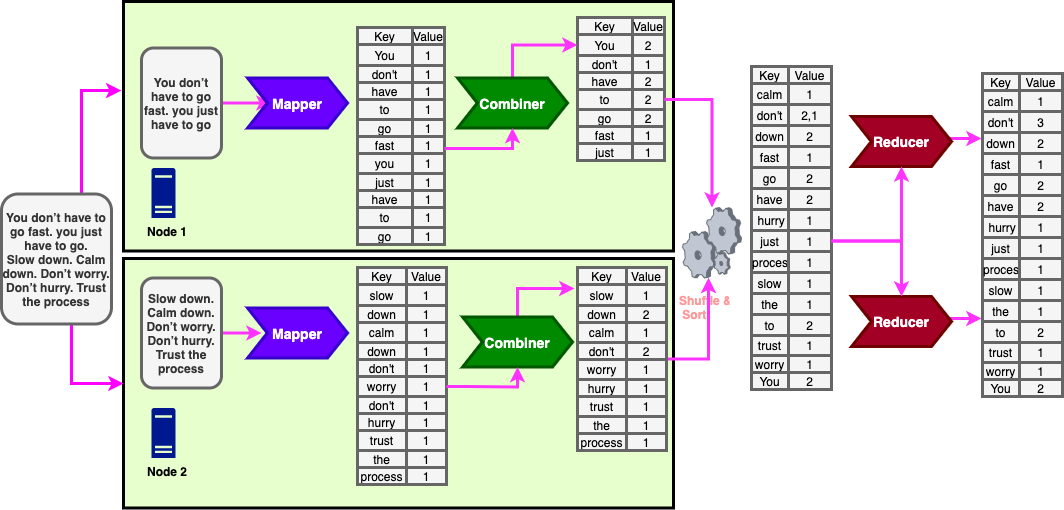
\includegraphics[height=.85\textheight]{./Figures/chapter-02/map-reduce-combiner-ex-2.png}
		\caption{Map Reduce Without Combiner } \label{fig:MRCombiner2}
	\end{figure}			
\end{frame}
%%%%%%%%%%%%%%%%%%%%%%%%%%%%%%%%%%%%%%%%%%%%%%%%%%%%%%
\begin{frame}[c]{ }
	\frametitle{Combiners Motivation }
	
	
	\begin{itemize}  [<+->]
		\item [--] Moving data between nodes is one of the bottlenecks in distributed systems.
		\item [--] 	We need to find always solutions to reduce the amount of data movement in the network.
		\item [--] In most cases, mappers produce large amounts of intermediate data passed on to the reducers for further processing. This leads to enormous network congestion.
		\item [--] One of the solutions is to reduce the mapper output using combiners. using \textbf{\underline{\textit{combiners "mini-reducer".}}}
		
	\end{itemize}
\end{frame}
%%%%%%%%%%%%%%%%%%%%%%%%%%%%%%%%%%%%%%%%%%%%%%%%%%%%%%
\begin{frame}[c]{ }
	\frametitle{How Combiner Works? }
	
	
	\begin{itemize}  [<+->]
		\item [--] The combiner must implement the \code{Reducer} interface’s \code{reduce()} method.
		
		\item [--] The combiner process on each map output key \& value (same as the Reducer). 

	\end{itemize}
\end{frame}

%%%%%%%%%%%%%%%%%%%%%%%%%%%%%%%%%%%%%%%%%%%%%%%%%%%%%%
\begin{frame}[c]{ }
	\frametitle{Combiners and Reducers }
	
	Combiner and Reducer code are often identical. 
	\begin{itemize}  [<+->]
	
	\item [--] Combiner \& Reducer must have identical input and output data types.
	
	\item [--] The operation must be  commutative and associative.
	\end{itemize}
\end{frame}

%%%%%%%%%%%%%%%%%%%%%%%%%%%%%%%%%%%%%%%%%%%%%%%%%%%%%%
\begin{frame}[c]{ }
	\frametitle{Combiners and Reducers }
	
	\begin{itemize}  [<+->]
		
		\item [--] \color{yellow}{ \textbf{\underline{\textit{Combiner runs on the Map-Side.}}}}
		
		\item [--] The output of the Combiner passed to the Reducer.
	\end{itemize}
\end{frame}
%%%%%%%%%%%%%%%%%%%%%%%%%%%%%%%%%%%%%%%%%%%%%%%%%%%%%%
\begin{frame}[c]{ }
	\frametitle{Associative and Commutative }
	
	\begin{itemize}  [<+->]
		
		\item [--] In math, the associative and commutative properties are laws applied to addition and multiplication that always exist.
		
				
	\end{itemize}
\footnotetext[1]{This example taken from  \href{https://sciencing.com/associative-commutative-property-of-addition-multiplication-with-examples-13712459.html}{https://sciencing.com/associative-commutative-property-of-addition-multiplication-with-examples-13712459.html}	} 
\end{frame}
%%%%%%%%%%%%%%%%%%%%%%%%%%%%%%%%%%%%%%%%%%%%%%%%%%%%%%
\begin{frame}[c]{ }
	\frametitle{Associative and Commutative }

	\begin{itemize}  [<+->]
		
		\item [--] In math, the associative and commutative properties are laws applied to addition and multiplication that always exist.
		
		
	\end{itemize}

\footnotetext[1]{This example taken from  \href{https://sciencing.com/associative-commutative-property-of-addition-multiplication-with-examples-13712459.html}{https://sciencing.com/associative-commutative-property-of-addition-multiplication-with-examples-13712459.html}	} 
\end{frame}
%%%%%%%%%%%%%%%%%%%%%%%%%%%%%%%%%%%%%%%%%%%%%%%%%%%%%%
\begin{frame}[c]{ }
	\frametitle{Associative and Commutative }
	\begin{itemize}  [<+->]
	
	\item [--] The associative property states that you can re-group numbers and you will get the same answer.
	
	
\end{itemize}

\begin{gather*}	
a + (b + c) =  (a + b) + c \\
1 + (2 + 3) = (1 + 2) + 3
\end{gather*}
\begin{gather*}
a \times (b \times c) =  (a \times b) \times c \\
1 \times (2 \times 3) =  (1 \times 2) \times 3
\end{gather*}

\footnotetext[1]{This example taken from  \href{https://sciencing.com/associative-commutative-property-of-addition-multiplication-with-examples-13712459.html}{https://sciencing.com/associative-commutative-property-of-addition-multiplication-with-examples-13712459.html}	} 
\end{frame}
%%%%%%%%%%%%%%%%%%%%%%%%%%%%%%%%%%%%%%%%%%%%%%%%%%%%%%
\begin{frame}[c]{ }
	\frametitle{Associative and Commutative }
	\begin{itemize}  [<+->]		
		\item [--] The commutative property states that you can move numbers around and still arrive at the same answer.	
	\end{itemize}


\begin{gather*}	
	a + b =  b + a \\
	1 + 2 = 2 + 1
\end{gather*}
\begin{gather*}
	a \times b =  b \times a \\
	1 \times 2 \times =  2 \times 1
\end{gather*}

\footnotetext[1]{This example taken from  \href{https://sciencing.com/associative-commutative-property-of-addition-multiplication-with-examples-13712459.html}{https://sciencing.com/associative-commutative-property-of-addition-multiplication-with-examples-13712459.html}	} 
\end{frame}
%%%%%%%%%%%%%%%%%%%%%%%%%%%%%%%%%%%%%%%%%%%%%%%%%%%%%%
\begin{frame}[c]{ }
	\frametitle{Combiners and Reducers }
	\begin{itemize}  [<+->]		
		\item [--] Reducers maybe used as Combiners if the operation is associative and commutative.	
	\end{itemize}


\end{frame}
%%%%%%%%%%%%%%%%%%%%%%%%%%%%%%%%%%%%%%%%%%%%%%%%%%%%%%
%%%%%%%%%%%%%%%%%%%%%%%%%%%%%%%%%%%%%%%%%%%%%%%%%%%%%%
\begin{frame}[c]{ }
	\frametitle{Combiners and Reducers }
	
\begin{figure}
	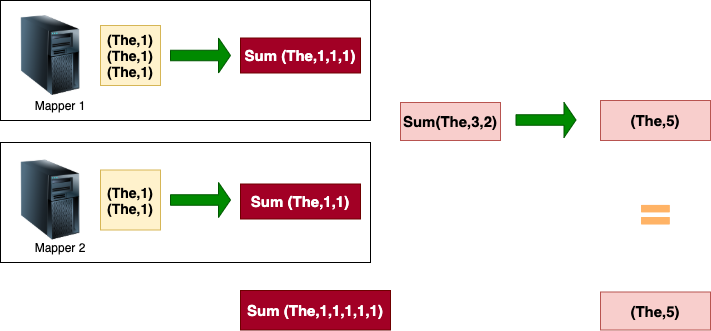
\includegraphics[height=.7\textheight]{./Figures/chapter-02/Combiners.png}
	\caption{Associative and Commutative Example }
\end{figure}		
\end{frame}
%%%%%%%%%%%%%%%%%%%%%%%%%%%%%%%%%%%%%%%%%%%%%%%%%%%%%%
\begin{frame}[c]{ }
	\frametitle{Combiners and Reducers }
	
	\begin{figure}
		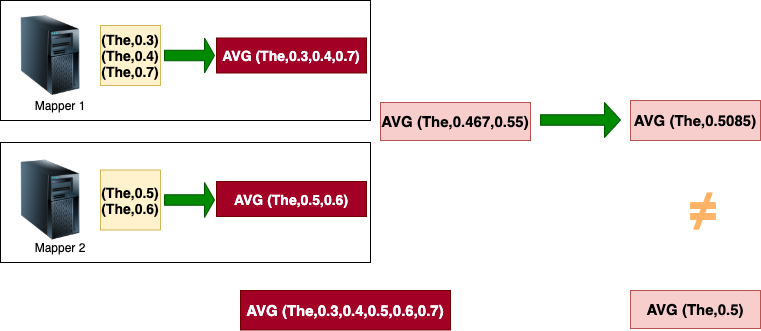
\includegraphics[height=.7\textheight]{./Figures/chapter-02/Combiners_AVG.png}
		\caption{Associative and Commutative Example }
	\end{figure}		
\end{frame}

